% Shared preamble for the English summaries in this repository.
\documentclass[11pt,a4paper]{article}
\usepackage[margin=2.2cm]{geometry}
\usepackage[T1]{fontenc}
\usepackage[utf8]{inputenc}
\usepackage{lmodern}
\usepackage{amsmath,amssymb}
\usepackage{graphicx}
\usepackage{booktabs}
\usepackage{enumitem}
\usepackage[hidelinks]{hyperref}
\setlist{itemsep=2pt,topsep=4pt}
\setlength{\parindent}{0pt}
\setlength{\parskip}{5pt}
\graphicspath{{figures/}}
\newcommand{\summaryheader}[3]{%
  \begin{center}
    {\Large\bfseries #2}\\[3pt]
    {\large #1}\\[3pt]
    {\small Arshia Goshtasbi \textbullet{} MSc Electrical Engineering (Control), Iran University of Science and Technology \textbullet{} #3}
  \end{center}
  \vspace{2pt}\hrule\vspace{8pt}
  \noindent\textit{English summary of my original Persian report, which is kept as a PDF in this folder.}\par}

\begin{document}
\summaryheader{Multivariable Control, Homework 2}{Representations, Pairing, and Decoupling a Distillation Column}{Autumn 1403 (2024)}

\section*{Questions}
\begin{itemize}
  \item \textbf{Transfer function versus state space.} Transfer functions are simple for linear SISO analysis and classical design, but they get unwieldy for MIMO systems, hide internal states and apply only to linear systems. State space handles MIMO, internal variables and nonlinear or time-varying models directly, at the price of matrix computations. I illustrated both with a mass--spring--damper.
  \item \textbf{Input--output pairing.} I described the relative gain array, $\Lambda(G)=G\circ(G^{-1})^T$, following Skogestad and Postlethwaite, and how to choose pairings from it, using the slide's reactor example.
  \item \textbf{MIMO design methods.} A short survey of state-space methods (LQR, state feedback), frequency-response and root-locus methods, pole placement, multivariable PID and robust control, each with an application example.
\end{itemize}

\section*{Simulation: a $2\times2$ distillation column}
The plant is
\[
G(s)=\frac{1}{75s+1}\begin{bmatrix}87.8 & -86.4\\ 108.2 & -109.6\end{bmatrix},
\]
which is strongly interacting. I built four Simulink models and applied unit steps on $u_1$, $u_2$ and both together:
\begin{enumerate}
  \item open loop, to show the interaction (\texttt{Q1.slx});
  \item two independent PID loops tuned with \texttt{pidtune} on $G_{11}$ and $G_{22}$ (\texttt{Q2Code.m}, \texttt{Q2.slx});
  \item two PIDs with a dynamic decoupler $T_{12}=-G_{12}/G_{11}$, $T_{21}=-G_{21}/G_{22}$ (\texttt{Q3Code.m}, \texttt{Q3.slx});
  \item an inverse decoupler with integral action (\texttt{Q4.slx}).
\end{enumerate}
Without decoupling, the two loops interact clearly. Decoupling largely removes the cross-coupling, and the inverse decoupler with integral action gives the smoothest responses.

\begin{center}
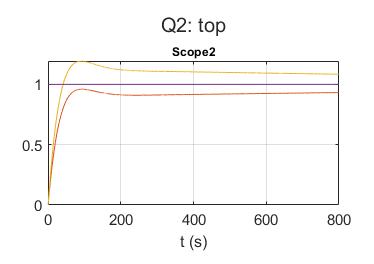
\includegraphics[width=0.32\linewidth]{Q2_scopes.png}\hfill
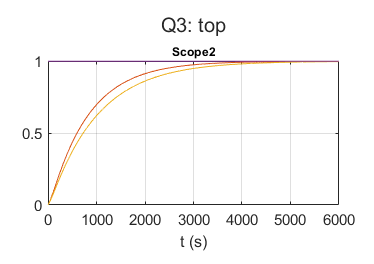
\includegraphics[width=0.32\linewidth]{Q3_scopes.png}\hfill
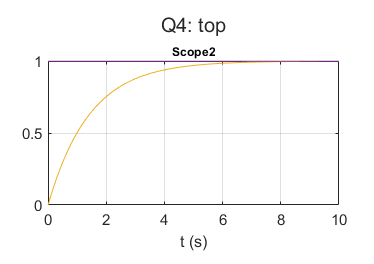
\includegraphics[width=0.32\linewidth]{Q4_scopes.png}\\[2pt]
{\small Re-run in R2023b, steps on both inputs. Left: independent PIDs. Middle: with the decoupler. Right: inverse decoupler with integrator.}
\end{center}
\end{document}
